\documentclass[12pt]{article}

%-------------PACKAGES------------- 
\usepackage[margin=1in]{geometry} 
\usepackage{amsmath,amsthm,amssymb}
\usepackage{pgfplots}
\usepackage{float}
\usepackage{braket}
\usepackage{titling}
\usepackage{wrapfig}
\usepackage{tikz}
\usepackage{mwe}
\usepackage{enumitem}
\usepackage{mathtools}
\usepackage{scrextend}
\usepackage{listings}
\usepackage{color}
\usepackage{caption}
\usepackage{subcaption}
\usepackage{algorithm,algpseudocode}
\usetikzlibrary{shapes,arrows,chains}
\usetikzlibrary[calc]

%-------------FORMATTING-------------
\setlength{\droptitle}{-7.5em} 
\setlength{\parindent}{0pt}
\def\LW{\dimexpr.25\linewidth-.5em} 
\tikzstyle{line} = [draw, -latex']
 
%--------------COMMANDS--------------
\newcommand{\N}{\mathbb{N}}
\newcommand{\Z}{\mathbb{Z}}
\newcommand{\R}{\mathbb{R}}
\newcommand{\C}{\mathbb{C}}
%\renewcommand{\qedsymbol}{\filledbox}

\DeclarePairedDelimiter \abs{\lvert}{\rvert}%
\DeclarePairedDelimiter \babs{\bigg\lvert}{\bigg\rvert}%
\DeclarePairedDelimiter \norm{\lVert}{\rVert}%

%------------ENVIRONMENTS------------- 
\newenvironment{theorem}[2][]{\begin{trivlist}
\item[{\bfseries #1}\hskip \labelsep {\bfseries #2.}]}{\end{trivlist}}
\newenvironment{lemma}[2][Lemma]{\begin{trivlist}
\item[\hskip \labelsep {\bfseries #1}\hskip \labelsep {\bfseries #2.}]}{\end{trivlist}}
\newenvironment{exercise}[2][Exercise]{\begin{trivlist}
\item[\hskip \labelsep {\bfseries #1}\hskip \labelsep {\bfseries #2.}]}{\end{trivlist}}
\newenvironment{reflection}[2][Reflection]{\begin{trivlist}
\item[\hskip \labelsep {\bfseries #1}\hskip \labelsep {\bfseries #2.}]}{\end{trivlist}}
\newenvironment{proposition}[2][Proposition]{\begin{trivlist}
\item[\hskip \labelsep {\bfseries #1}\hskip \labelsep {\bfseries #2.}]}{\end{trivlist}}
\newenvironment{corollary}[2][Corollary]{\begin{trivlist}
\item[\hskip \labelsep {\bfseries #1}\hskip \labelsep {\bfseries #2.}]}{\end{trivlist}}
\newenvironment{definition}[2][]{\begin{trivlist}
\item[{\bfseries #1}\hskip \labelsep {\bfseries #2.}]}{\end{trivlist}}
\theoremstyle{remark}
\newtheorem*{remark}{Remark}

%-------------CODE-STYLE------------
\definecolor{dkgreen}{rgb}{0,0.6,0}
\definecolor{gray}{rgb}{0.5,0.5,0.5}
\definecolor{mauve}{rgb}{0.58,0,0.82}
\lstset{frame=tb,
	language=C++,
	aboveskip=3mm,
	belowskip=3mm,
	showstringspaces=false,
	columns=flexible,
	basicstyle={\small\ttfamily},
	numbers=none,
	numberstyle=\tiny\color{gray},
	keywordstyle=\color{blue},
	commentstyle=\color{dkgreen},
	stringstyle=\color{mauve},
	breaklines=true,
	breakatwhitespace=true,
	tabsize=3
}

\tikzset{
	path image/.style={
		path picture={
			\node at (path picture bounding box.center) {
				\includegraphics[height=3cm]{example-image}};}},
	path tikzimage/.style={
		path picture={
			\node at (path picture bounding box.center)
			[circle, fill=blue!50, scale=2, text=yellow]{Bravo};}}
}
	
\lstset{
	morekeywords={end}
}

%------------------------------------ 
%---------START-OF-DOCUMENT----------
%------------------------------------
\begin{document}
 
\title{Paper Summary}
\author{David Miller \\ 
CIS 5930: Social Network Mining} 

\maketitle 

\begin{figure}[H]{}
	\centering
	\vspace{-15pt}
	\hspace{-10pt}
	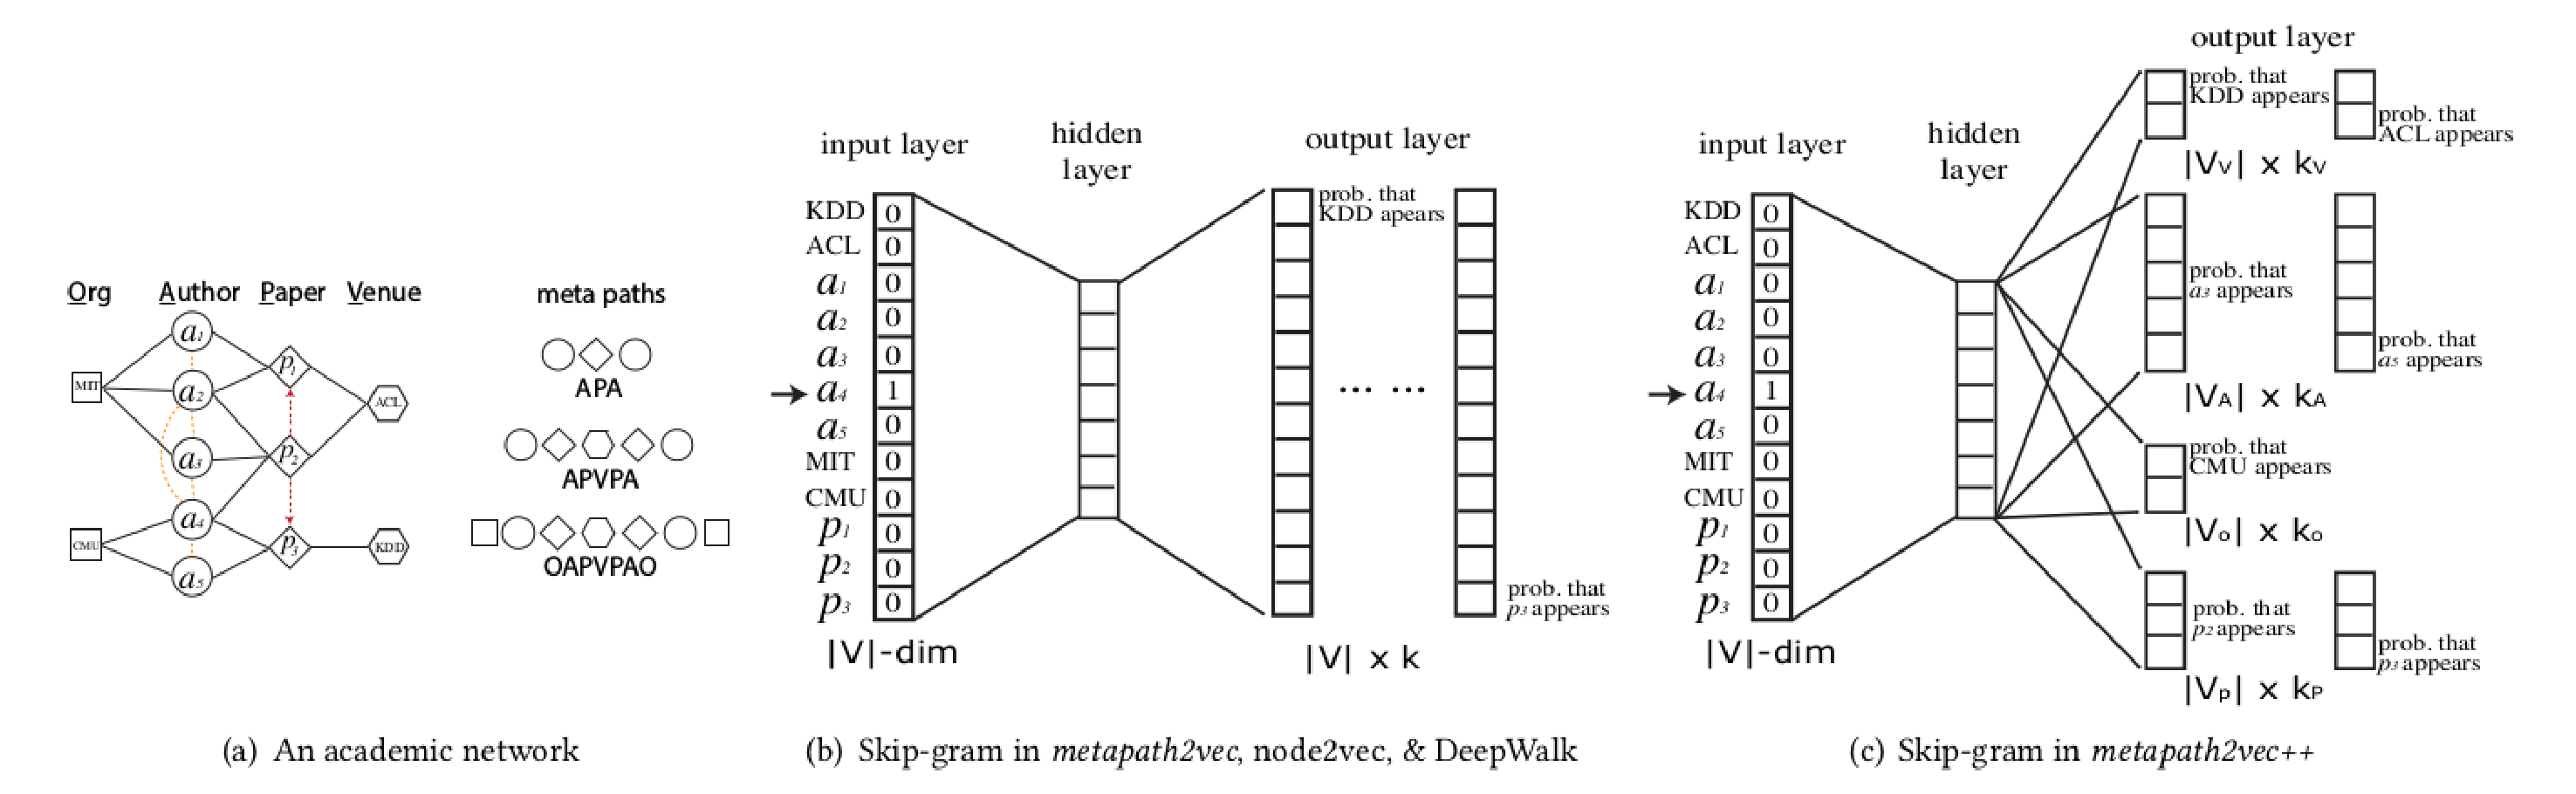
\includegraphics[height=5cm,width=1\textwidth]{fig1.eps}
	\caption{}
	\vspace{0pt}
\end{figure} 

A Heterogeneous Network is defined as a graph $G = (V , E,T )$ in which each node $v$ and each link $e$ are associated with their mapping functions $\phi(v) : V \rightarrow T_V$ and $\phi(e) : E \rightarrow T_E$ ,
respectively. $T_V$ and $T_E$ denote the sets of object and relation types,
where $|T_V| + |T_E| > 2$ \cite{paper}. Given this definition, we can state the problem as follows:
\begin{definition}{Problem}
	Given a heterogeneous network $G$, the task is to learn the $d$-dimensional latent representations $X \in \mathbb{R}^{|V|d} , d << |V|$  that are able to capture the structural and semantic relations among them
\end{definition} 

What the problem is essentially stating given some input $I$ we try to find the best (lowest) dimension $d$ that accurately represent and captures the relationship amongst elements in $I$. \\ 

The problem generates similar neighborhoods based on random meta-paths $\mathcal{P}: V_1 \xrightarrow[]{R_1} V_2 \xrightarrow[]{R_2} \dots V_t \xrightarrow[]{R_t} V_{t+1} \dots \xrightarrow[]{R_{l-1}} V_l$, where $R_i$ is the relationship between nod $V_i$ and $V_{i+1}$ and where probability of transition is given by 
\begin{align*}
	p(v^{i+1} | v_t^i, \mathcal{P}) = 
	\begin{cases}
	\frac{1}{\abs{N_{t+1}(v_t^i)}} & (v^{i+1}, v_t^i) \in E, \phi(v^{i+1}) = t+1) \\
	0 & (v^{i+1}, v_t^i) \in E, \phi(v^{i+1}) \neq t+1 \\
	0 & \not\in E	
	\end{cases}
\end{align*}
which essentially states that the walker is likely to go to a node within its neighborhood. Once all nodes on the neighborhood have been visited, there is no place for the random walker to go and thus this creates a neighborhood of some shared context. This is essentially what \textit{metapath2vec} does. What \textit{metapath2vec++} does it just add probability distributions to context types $c_1, \dots, c_t$ to increases neighborhood classification. Future work is discussed very well in the paper. It includes different improvements and optimizations that can be done: optimizing sampling space, machine learning to uncover meaningful meta-paths, allow the model to work with dynamic data, and generalizing the model for all types of heterogeneous networks.  

\newpage

Three strengths I found with the paper are
\begin{enumerate}
	\item \textit{metapath2vec} and \textit{metapath2vec++} models are efficient and scalable for large-scale heterogeneous networks with millions of nodes \cite{paper}.
	\item The area of application lends itself well to data visualization, allowing for easy communication with the public and possible commercial consumers if sold as a product.
	\item Parameter sensitivity allows contexts to be weighted respective to their significance.
\end{enumerate} 
\vspace{0.5cm}

Three weaknesses I found with the paper are
\begin{enumerate}
	\item A lack of applications; the paper (results including) focused too much on the author and venue networks.
	\item There was no evidence suggesting that this can be applied to GPU computing, which I believe to be an appropriate computing venue for \textit{metapath2vec} and \textit{metapath2vec}.
	\item Lack of analysis. Topics such as statistics and probability deserve a thorough analysis to provide evidence that algorithms based on them are valid and reliable. There is a lack of this sort of analysis in the paper. 
\end{enumerate}
\vspace{0.5cm}

Questions for the reader
\begin{enumerate}
	\item What exactly does \textit{metapath2vec++} offer over \textit{metapath2vec}?
	\item Is there a way to embed the data in one dimension while keeping context of data?
	\item If machine learning is used for metapath finding, how would that work?
\end{enumerate}
\vspace{0.5cm}

\begin{thebibliography}{unsrt}
	\bibitem{paper}
	Yuxiao Dong, Nitesh V. Chawla, Ananthram Swami, \emph{metapath2vec: Scalable Representation Learning for Heterogeneous Networks}, KDD’17, August 13-17, 2017, Halifax, NS, Canada.
\end{thebibliography}

\end{document}